
\begin{figure}
    \centering
    \begin{subfigure}[b]{0.45\textwidth}
        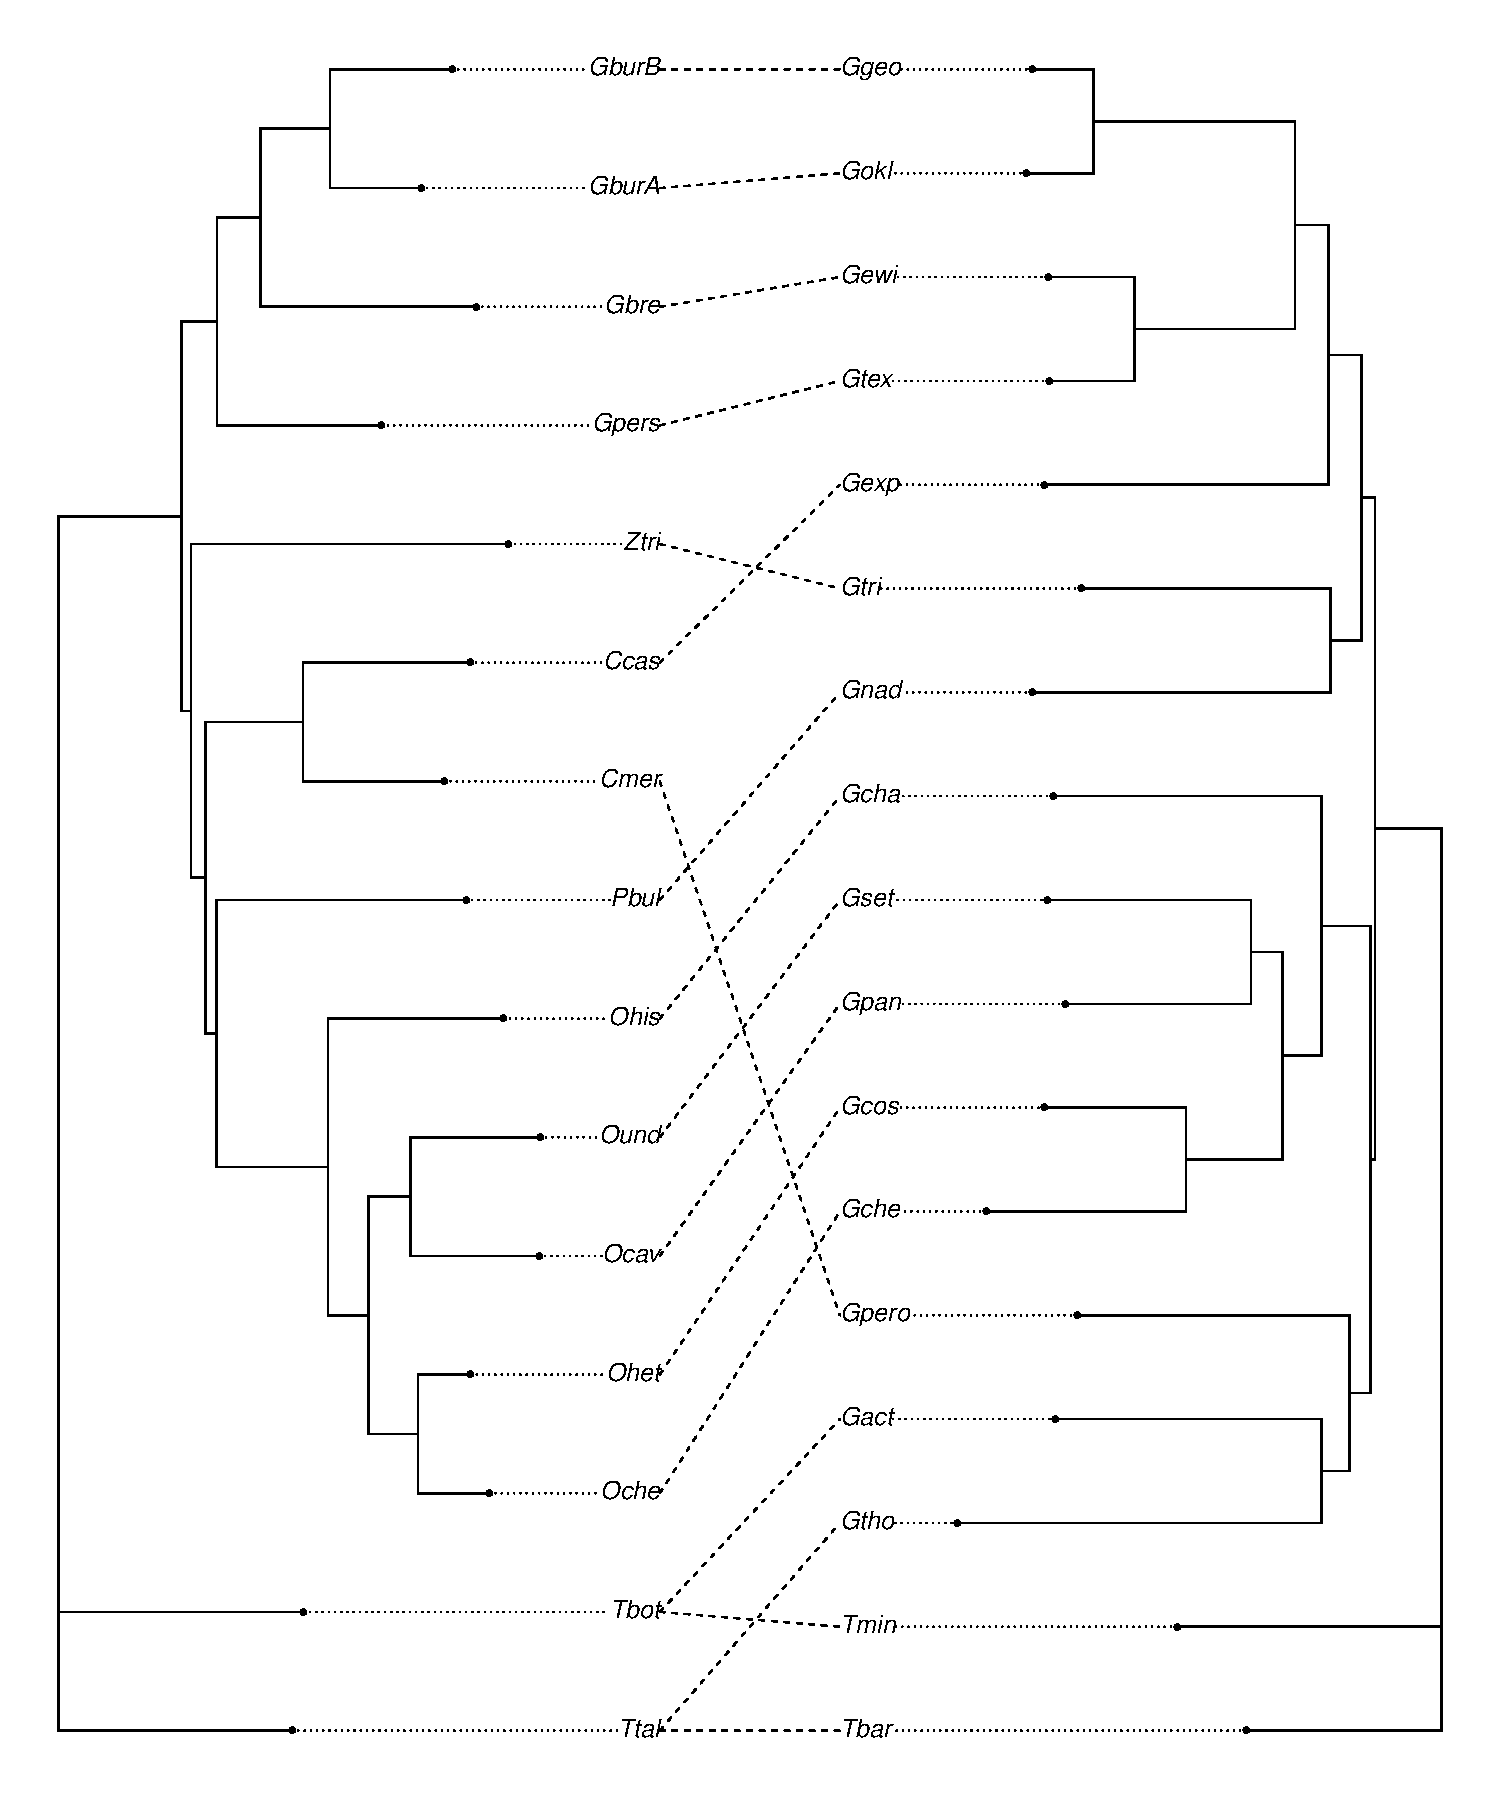
\includegraphics[width=\textwidth]{FishPoo/figures/codiv_gopher_louse}
        \small
        \caption{Gopher/Louse}
    \end{subfigure}
    \begin{subfigure}[b]{0.45\textwidth}
        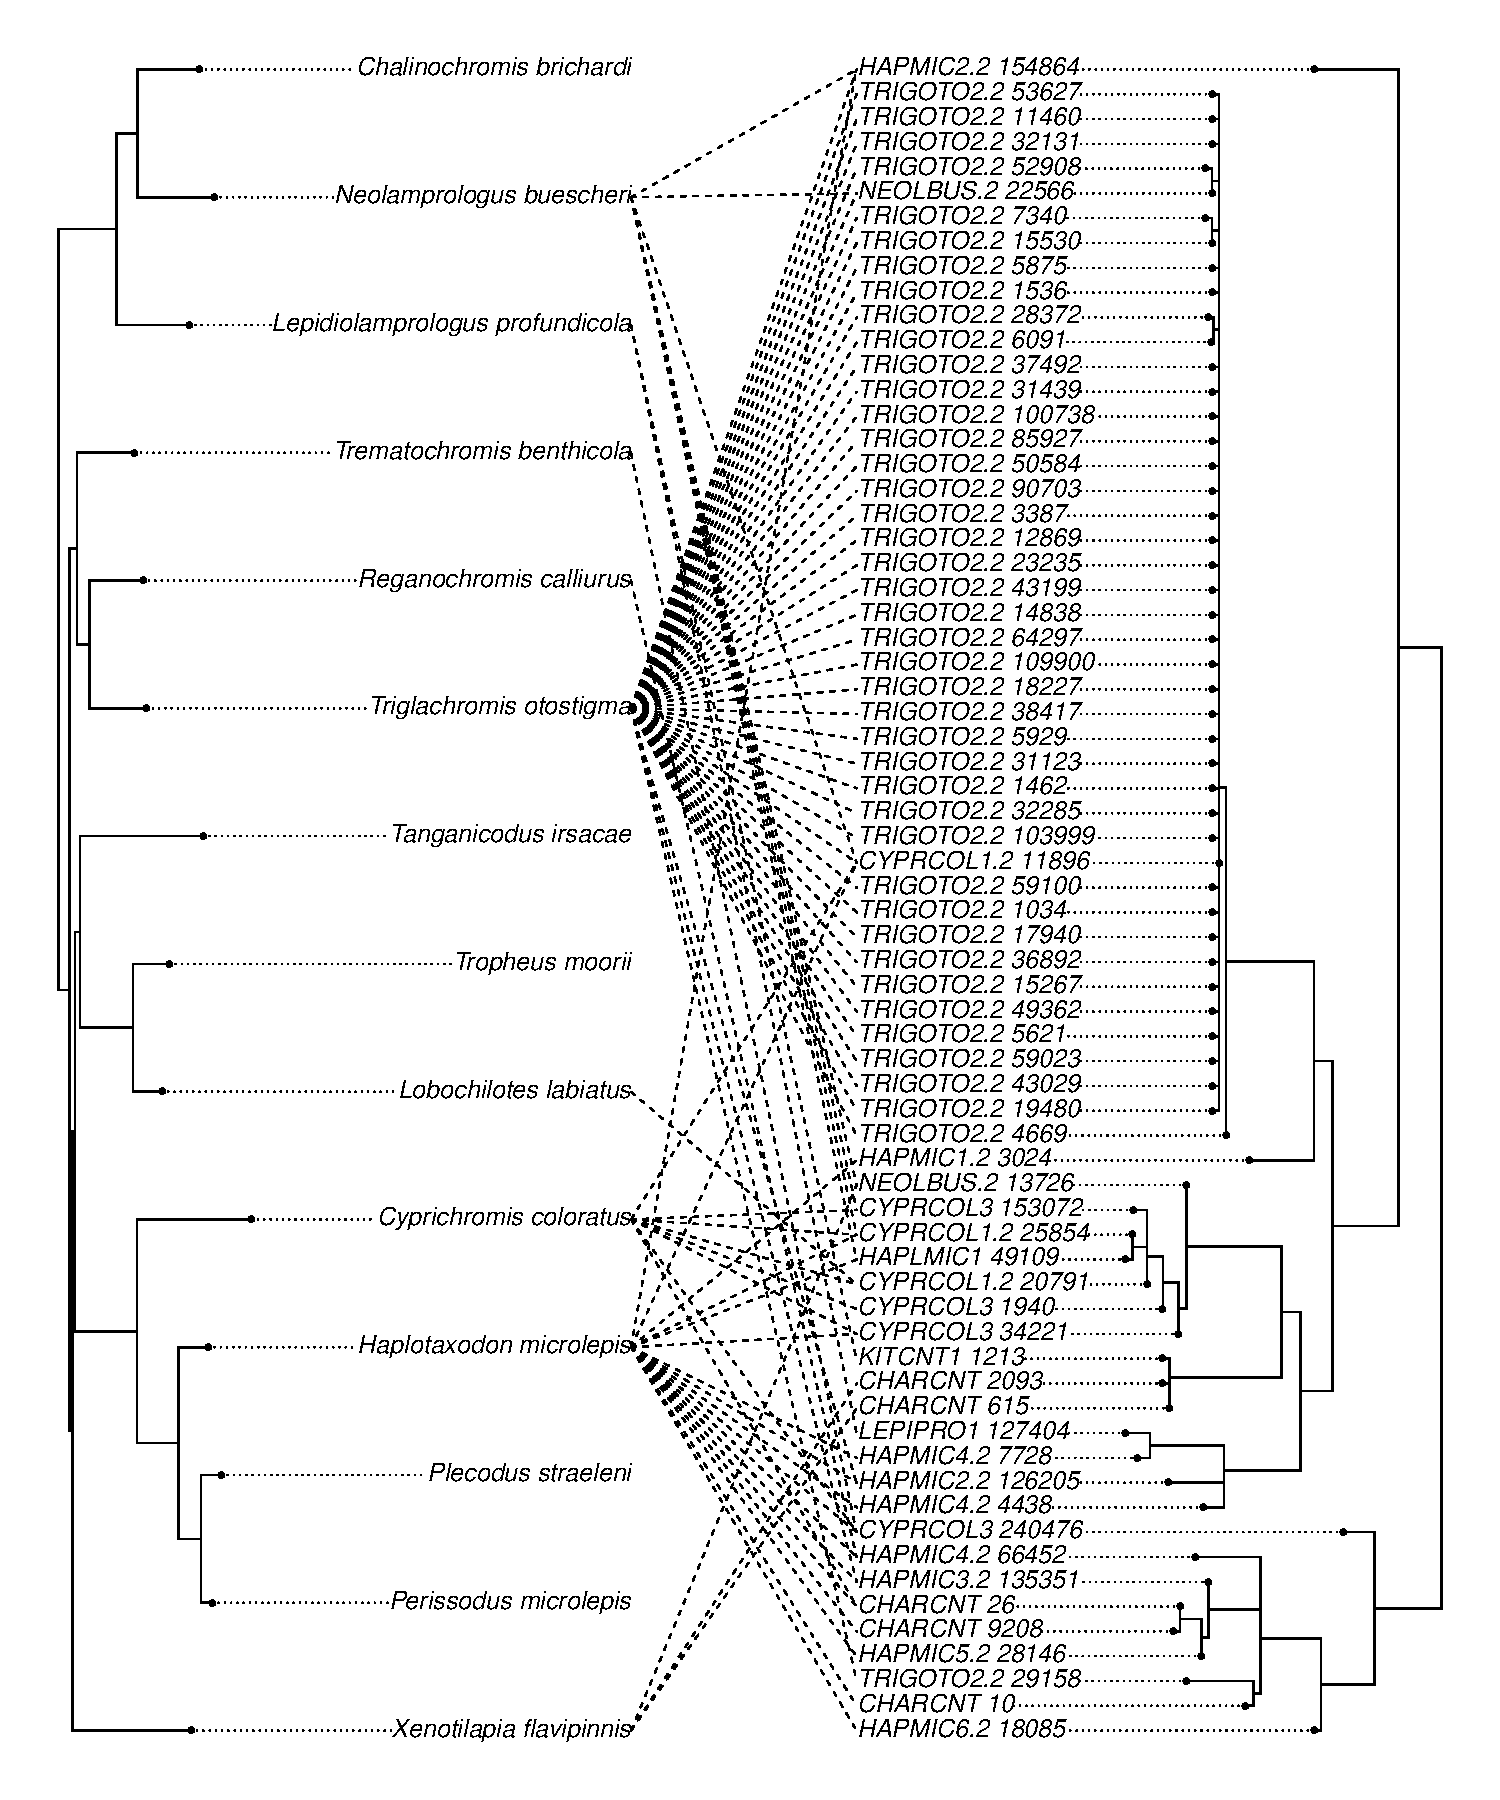
\includegraphics[width=\textwidth]{FishPoo/figures/codiv_clade_72223}
        \small
        \caption{Clade 72223}
    \end{subfigure}\\
    \caption{Tanglegrams illustrating the interactions among pocket gophers and their chewing lice parasites from Hafner {\em et al.} \cite{hafner1994disparate} \textbf{(a)}, and Clade 72223, a group of OTUs associated with Tanganyikan cichild fishes \textbf{(b)}.}
    \label{fig:FP_tangles}
\end{figure}